%! TEX root = ../main.tex
\documentclass[main]{subfiles}

\begin{document}
\chapter{Walsh関数を用いた代理モデル}
    前章で,先行研究の課題に計算時間の長さが上げられた.
    本研究では高速な代理モデルを使い,SUMOによるシミュレートを代理することによって計算時間の短縮を図る.
    本研究で代理モデルとして用いるWalsh関数について述べる.

    \section{Walsh関数}   
    Walsh関数\cite{walsh}は1923年にJ.L.Walshにより提唱された.
    Walsh関数は$n$個の入力$x \in \{0, 1\}, x_1, x_2, ..., x_n$の時,式\ref{walsh_siki}で表される.
    \begin{equation}
        \begin{split}
            f(x_1, x_2, ..., x_n) &= w_1(-1)^{x_1} + w_2(-1)^{x_2} + ... + w_n(-1)^{x_n} \\
            &+ w_{12}(-1)^{x_1+x_2} + ... + w_{n-1n}(-1)^{x_{n-1}+x_n} \\
            &+ w_{123}(-1)^{x_1+x_2+x_3} + ... + w_{n-2n-1n}(-1)^{x_{n-2}+x_{n-1}+x_n} \\
            &+ ...
            \label{walsh_siki}
        \end{split}
    \end{equation}
    
    Walsh関数はそれぞれの入力値を-1に累乗し,パラメータwを掛け,その和を返す関数である.
    このパラメータ$w$は未知であり,データを学習することによって決定する.
    式\ref{walsh_siki}の1行目は入力値の一つが指数にかかっている.よって1行目の項数は$n$である.
    それに対し,2行目は$x_1+x_2$というように入力値の2つの和が指数にかかっている.よって2行目の項数は${}_n \mathrm{C}_2$となる.
    同様に,3行目は$x_1+x_2+x+3$というように入力値の3つの和が指数にかかっている.よって3行目の項数は${}_n \mathrm{C}_3$となる.
    このように,Walsh関数は入力値を組み合わせた和を指数にするという特徴がある.
    そこで,Walsh関数が入力値をいくつ組み合わせているかをOrderで表すようにする.
    式\ref{walsh_siki}の1行目はOrder1,2行目はOrder2となる.
    Walsh関数は完全正規直行基底を構成しており,Order$n\to \infty$の時,任意の関数を表現することが出来る.
    ただし,実際にWalsh関数を利用する際は,このOrderを無限にすることはできない.
    また,Order$k$の時の項数は${}_n \mathrm{C}_k$となり,その計算量オーダーは$\mathcal{O}(n!)$となる.
    そのため,kの値を一つ増やすだけで全体の項数が大きく増え,計算時間が大きくかかってしまうため,
    使用するWalsh関数のOrderを考慮することが重要である.

    \section{代理モデル}
    学習済みのWalsh関数で入力値から出力値を得ることは数秒もかからない.
    入力値から出力値を得ることに約40分かかるSUMOと比較すると圧倒的に高速である.
    よって,SUMOによる運行スケジュールとその出力である総移動時間と乗車率をWalsh関数により学習させ,
    代理モデルとしてSUMOの代わりに使用することで実験の高速化が可能だと考えられる.
    図\ref{dairi}にシミュレートの代わりに代理モデルを使用する際のイメージ図を示す.
    \begin{figure}
        \centering
        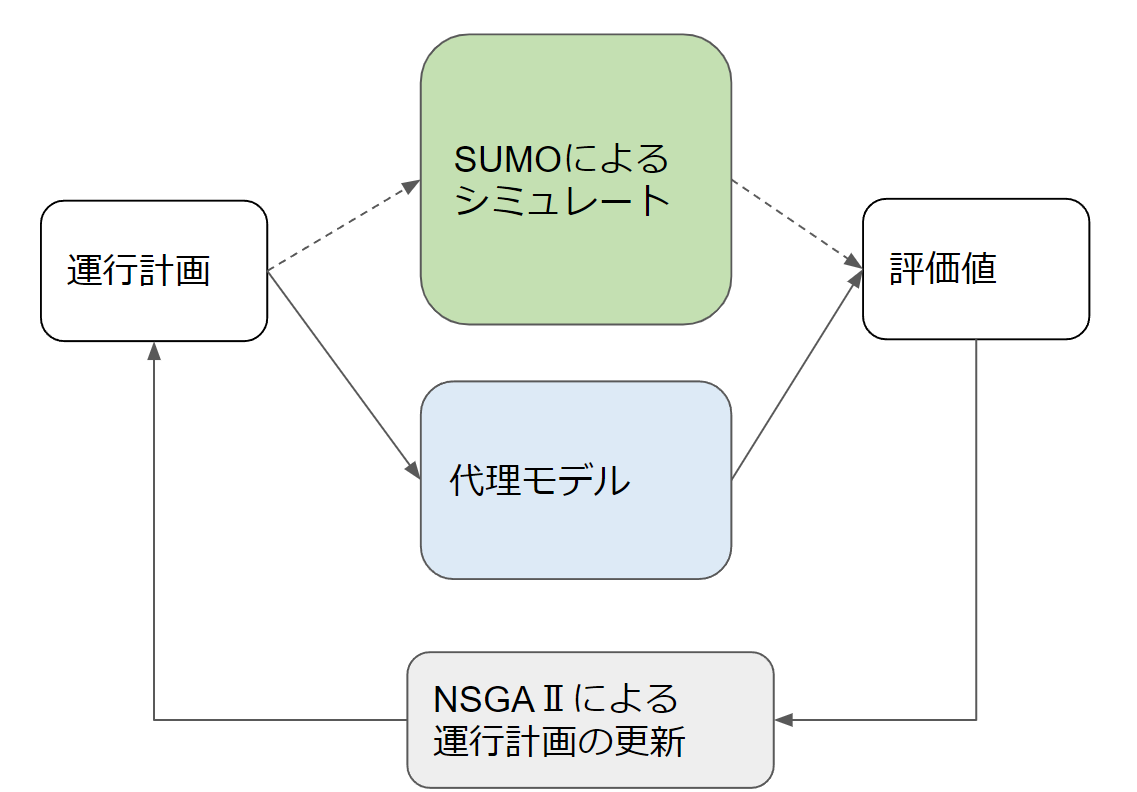
\includegraphics[width=\linewidth]{figures/dairi.png}
        \caption{代理モデルの導入イメージ}
        \label{dairi}
    \end{figure}



\end{document}